\begin{table*}[tb]
    \centering
    \begin{adjustbox}{width=2\columnwidth,center}
		\begin{tabular}{l|l|l|c|c|c|c|c|c|c|c}
			\toprule
			\multirow{3}{0.02\linewidth}{OOD detector} & \multirow{3}{0.13\linewidth}{Hyperparameters} &
			\multirow{3}{0.07\linewidth}{ $\eta^{}_{\bff}(\bfC)$} & \multicolumn{8}{c}{OOD data} \\ \cline{4-11}
    		& & & \multicolumn{2}{c|}{\texttt{Places}} & \multicolumn{2}{c|}{\texttt{SUN}} & \multicolumn{2}{c|}{\texttt{Textures}} & \multicolumn{2}{c}{\texttt{iNaturalist}}\\ \cline{4-11}
    		& & & $\eta^{}_{\bff, S}(\bfC)$ & J_{\textrm{sep}}(\bfC, \bfC') & $\eta^{}_{\bff, S}(\bfC)$ & J_{\textrm{sep}}(\bfC, \bfC') & $\eta^{}_{\bff, S}(\bfC)$ & J_{\textrm{sep}}(\bfC, \bfC') & $\eta^{}_{\bff, S}(\bfC)$ & J_{\textrm{sep}}(\bfC, \bfC') \\ \hline \hline
			\multirow{4}{0.10\linewidth}{MSP} 
			& $\lambda_\textrm{mse} = 0, \lambda_\textrm{norm} = 0, \lambda_\textrm{sep} = 0$ & 0.990 & 0.849 & 0.0 & 0.848 & 0.0 & 0.824 & 0.0 & 0.958 & 0.0\\
			& $\lambda_\textrm{mse} = 10, \lambda_\textrm{norm} = 0.1, \lambda_\textrm{sep} = 0$ & \textbf{0.994} & 0.947 &0.216 & 0.946 & 0.118 & 0.922 & \textbf{0.406} & \textbf{0.970} & 0.175 \\
			& $\lambda_\textrm{mse} = 0, \lambda_\textrm{norm} = 0, \lambda_\textrm{sep} = 50$ & 0.980 & 0.815 & \textbf{0.412} & 0.816 & \textbf{0.303} & 0.773 & 0.376 & 0.863 & 0.267\\
			& $\lambda_\textrm{mse} = 10, \lambda_\textrm{norm} = 0.1, \lambda_\textrm{sep} = 50$ & 0.985 & \textbf{0.959} & 0.327 & \textbf{0.961} & 0.266 & \textbf{0.938} & 0.344 & 0.946 & \textbf{0.286}\\ \hline 
			\multirow{4}{0.10\linewidth}{ODIN} 
			& $\lambda_\textrm{mse} = 0, \lambda_\textrm{norm} = 0, \lambda_\textrm{sep} = 0$ & 0.990 & 0.869 & 0.0 & 0.869 & 0.0 & 0.850 & 0.0 & 0.981 & 0.0\\
			& $\lambda_\textrm{mse} = 10^8, \lambda_\textrm{norm} = 0.1, \lambda_\textrm{sep} = 0$ & \textbf{0.994} & 0.951 & 0.161 & 0.959 & 0.215 & 0.936 & 0.411 & 0.936 & 0.151\\
			& $\lambda_\textrm{mse} = 0, \lambda_\textrm{norm} = 0, \lambda_\textrm{sep} = 50$ & 0.987 & 0.899 & \textbf{0.373} & 0.911 & 0.342 & 0.790 & \textbf{0.414} & 0.970 & \textbf{0.337}\\
			& $\lambda_\textrm{mse} = 0, \lambda_\textrm{norm} = 0, \lambda_\textrm{sep} = 0$ & 0.991 & \textbf{0.973} & 0.355 & \textbf{0.969} & \textbf{0.356} & \textbf{0.945} & 0.405 & \textbf{0.982} & 0.308 \\ \hline
			\multirow{4}{0.10\linewidth}{Energy} 
			& $\lambda_\textrm{mse} = 0, \lambda_\textrm{norm} = 0, \lambda_\textrm{sep} = 0$ & 0.990 & 0.845 & 0.0 & 0.847 & 0.0 & 0.832 & 0.0 & 0.973 & 0.0\\
			& $\lambda_\textrm{mse} = 1, \lambda_\textrm{norm} = 0.1, \lambda_\textrm{sep} = 0$ & \textbf{0.993} & 0.965 & 0.135 & 0.963 & 0.127 & 0.960 & 0.284 & 0.949 & 0.215\\
			& $\lambda_\textrm{mse} = 0, \lambda_\textrm{norm} = 0, \lambda_\textrm{sep} = 50$ & 0.987 & 0.779 & \textbf{0.422} & 0.794 & 0.371 & 0.767 & \textbf{0.510} & 0.911 & \textbf{0.288} \\
			& $\lambda_\textrm{mse} = 1, \lambda_\textrm{norm} = 0.1, \lambda_\textrm{sep} = 50$ & 0.990 & \textbf{0.971} & 0.365 & \textbf{0.970} & \textbf{0.400} & \textbf{0.964} & 0.494 & \textbf{0.973} & 0.280\\ \hline
			\multirow{4}{0.10\linewidth}{Mahal} 
			& $\lambda_\textrm{mse} = 0, \lambda_\textrm{norm} = 0, \lambda_\textrm{sep} = 0$ & 0.990 & 0.860 & 0.0 & 0.860 & 0.0 & 0.831 & 0.0 & 0.972 & 0.0 \\
			& $\lambda_\textrm{mse} = 0.1, \lambda_\textrm{norm} = 0.1, \lambda_\textrm{sep} = 0$ & \textbf{0.994} & 0.962 & 0.153 & 0.963 & 0.176 & 0.962 & 0.351 & 0.955 & 0.169\\
			& $\lambda_\textrm{mse} = 0, \lambda_\textrm{norm} = 0, \lambda_\textrm{sep} = 50$ & 0.985 & 0.850 & \textbf{0.430} & 0.883 & 0.362 & 0.774 & \textbf{0.429} & 0.926 & \textbf{0.386} \\
			& $\lambda_\textrm{mse} = 0.1, \lambda_\textrm{norm} = 0.1, \lambda_\textrm{sep} = 50$ & 0.991 & \textbf{0.971} & 0.370 & \textbf{0.970} & \textbf{0.388} & \textbf{0.970} & 0.397 & \textbf{0.972} & 0.351 \\ \bottomrule
		\end{tabular}
	\end{adjustbox}
	\caption[]{\small \textbf{Results of concept learning with different parameter settings across various OOD detectors and OOD datasets.} $\bfC'$ denotes a set of concepts discovered by baseline \cite{yeh2019completeness} (\ie $\lambda_\textrm{mse} = 0, \lambda_\textrm{norm} = 0, \lambda_\textrm{sep} = 0$).
	Note that by definition of $J_{\textrm{sep}}(\bfC, \bfC')$ (Eqn. \ref{eq:relative-separability}), $J_{\textrm{sep}}(\bfC, \bfC') = 0$ for baseline.
	By having $\lambda_\textrm{mse} > 0, \lambda_\textrm{norm} > 0, \lambda_\textrm{sep} = 0$, we observe that $\eta^{}_{\bff, S}(\bfC)$ is always improved by large margin compared to baseline.
	When $\lambda_\textrm{mse} = 0, \lambda_\textrm{norm} = 0, \lambda_\textrm{sep} > 0$, $J_{\textrm{sep}}(\bfC, \bfC')$ is maximized the most, but $\eta^{}_{\bff, S}(\bfC)$ is not enhanced or even degraded.
	Finally, with $\lambda_\textrm{mse} > 0, \lambda_\textrm{norm} > 0, \lambda_\textrm{sep} > 0$ when all of our regularization terms are considered, we achieve the best detection completeness in most of the cases.
	To encourage both detection completeness and concept separability, we have to sacrifice $J_{\textrm{sep}}(\bfC)$ a bit, but it is still a noticeable improvement compared to baseline.
	\textbf{Bold} numbers are superior results.}
	\label{tab:concept-learning-results}
\end{table*}

\section{Experiments}
\subsection{Setup}
\textbf{Dataset.} For the ID dataset, we use Animals with Attributes (AwA) \cite{xian2018awa} with 50 animal classes, and split it into train set (29841 images), validation set (3709 images), and test set (3772 images).
For OOD datasets, we use the MSCOCO dataset \cite{lin2014mscoco} as $\Douttr$.
For the OOD test dataset $\Doutte$ at test time, we follow a common setting in literature of large-scale OOD detection and use four different datasets: \texttt{Places365} \cite{zhou2017places}, \texttt{SUN} \cite{xiao2010sun}, \texttt{Textures} \cite{cimpoi2014textures}, \texttt{iNaturalist} \cite{van2018inaturalist}, all resized to $224 \times 224$ input shape.

% \jihye{real-world high resolution image data}
\textbf{DNN classifier.} To follow common setup in prior works \cite{yeh2019completeness, ghorbani2019ace, koh2020concept-bottleneck, kim2018tcav}, we test our method to interpret the widely-used Inception-V3 model \cite{szegedy2016inception-v3} trained on AwA, which yields $0.921$ test accuracy. 
For interpretation, we choose a layer right before the global max-pooling layer. 

\textbf{OOD detector.} We apply our general approach to intepret four popular OOD detection methods in the literature: MSP \cite{hendrycks2016msp}, ODIN \cite{liang2018ODIN}, Energy \cite{liu2020energy} and Mahalanobis \cite{lee2018mahalanobis} (henceforth abbreviated to Mahal). 

\textbf{Hyperparameters.}
In the following sections, all results are from applying different concept learning objectives to obtain $m = 100$ concepts (unless specifically mentioned otherwise). 
Following the implementation of \cite{yeh2019completeness}, we fix $\lambda_{\textrm{expl}} = 10$ throughout our experiments, set $\bfg$ to be a two-layer perceptron with $500$ neurons at hidden layer, and optimize using Adam \cite{kingma2014adam}.
We set the range of $\lambda_{\textrm{norm}}, \lambda_{\textrm{mse}}$ and $\lambda_{\textrm{sep}}$ (see Eqn. (\ref{equ: concept learning})) depending on the scale of corresponding terms (\ie $J_{\textrm{norm}}(\bfC),  J_{\textrm{mse}}(\bfC)$ and $ J_{\textrm{sep}}(\bfC)$, respectively) with a specific choice of OOD detector.
For ablation study to illustrate the effect of each parameter, see Appendix \ref{sec:appendix-concept-learning-ablation}\ryan{just adding a reminder to fill this in before submission}.
After concept learning with $m$ concepts, we remove duplicate concepts by removing those with a dot product of over $0.95$ with the others~\cite{yeh2019completeness}.

\subsection{Results}\label{subsec:results}
\mypara{Effectiveness of our concept learning objective.}
We test how effectively our regularization terms improve detection completeness and concept separability, without sacrificing the classification completeness.
In contrast to completeness scores that are close to the range $[0, 1]$ regardless of the choice of dataset, classification model or OOD detection algorithm, it is hard to gauge the possible range of separability score $J_{\textrm{sep}}(\bfC)$ (or $J^y_{\textrm{sep}}(\bfC)$) across different settings, and whether the resulted score is a meaningful improvement.
Hence, we devise a \textit{relative} concept separability that captures the relative improvement in concept separability between two different sets of concepts as
\begin{equation}
\label{eq:relative-separability}
J_{\textrm{sep}}(\bfC, \bfC') = \textrm{Median}\left(\left\{\frac{J^i_{\textrm{sep}}(\bfC) - J^i_{\textrm{sep}}(\bfC')}{J^i_{\textrm{sep}}(\bfC')}\right\}_{i=1}^L\right).   
\end{equation}
Eqn. (\ref{eq:relative-separability}) measures the median of the relative increase in the per-class separability $J^y_{\textrm{sep}}(\bfC)$ using concept $\bfC$, compared to $J^y_{\textrm{sep}}(\bfC')$ using another set of concept $\bfC'$.
We set $\bfC'$ to be the set of concepts learned by \cite{yeh2019completeness}, which is a special case of our learning objective when $\lambda_\textrm{mse} = 0, \lambda_\textrm{norm} = 0, \lambda_\textrm{sep} = 0$.
The set of concept $\bfC$ can be obtained via our concept learning with various combinations of hyperparameter choices.
For the full results of relative separability along with classification completeness and detection completeness across various OOD detectors and OOD datasets, refer to Table \ref{tab:concept-learning-results}.

Table \ref{tab:concept-learning-results} shows that $J_{\textrm{norm}}(\bfC)$ and $J_{\textrm{mse}}(\bfC)$ regularizers not only encourage the detection completeness, but also the classification completeness as well. 
This verifies our assumption that accurate reconstruction of feature representation space $\hat{\calZ}$ is beneficial for accurate explanations for both classifier and OOD detector.
Moreover, by having the separability regularizer $J_{\textrm{sep}}(\bfC)$, we improve the detection completeness even further, with better relative concept separability as well.

\begin{figure}[tbp]
\centering
\subfloat[MSP, target \label{fig:distr_msp_target}]{\includegraphics[width=0.15\textwidth]{figures/distr_msp_target.jpg}}\hfill
\subfloat[MSP, baseline \label{fig:distr_msp_yeh}] {\includegraphics[width=0.15\textwidth]{distr_msp_yeh.jpg}}\hfill
\subfloat[MSP, ours \label{fig:distr_msp_ours}]{\includegraphics[width=0.15\textwidth]{figures/distr_msp_ours.jpg}} \\
\subfloat[Energy, target\label{fig:distr_energy_target}]{\includegraphics[width=0.15\textwidth]{figures/distr_energy_target.jpg}}\hfill
\subfloat[Energy, baseline \label{fig:distr_energy_yeh}] {\includegraphics[width=0.15\textwidth]{figures/distr_energy_yeh.jpg}}\hfill
\subfloat[Energy, ours\label{fig:distr_energy_ours}]{\includegraphics[width=0.15\textwidth]{figures/distr_energy_ours.jpg}}
\caption{Estimated density of $S(\bfx, \cdot)$ between the AwA test data (ID; blue) and the SUN dataset (OOD; red). DNN classifier is Inception-V3 and OOD detector is either MSP \cite{hendrycks2016msp} or \cite{liu2020energy}.
\textbf{Left}: Target distribution of $S(\bfx, \bff)$ in canonical world. 
\textbf{Mid}: Distribution of $\Scon(\bfx, \bff)$ in concept world, using concepts learned by \cite{yeh2019completeness}.
\textbf{Right}: Distribution of $\Scon(\bfx, \bff)$ in concept world, using concepts learned by our method.
For MSP, we set $\lambda_\textrm{mse} = 10, \lambda_\textrm{norm} = 0.1, \lambda_\textrm{sep} = 0$ and for Energy, $\lambda_\textrm{mse} = 1, \lambda_\textrm{norm} = 0.1, \lambda_\textrm{sep} = 0$.}
\label{fig:score-distribution}
\end{figure}



\mypara{Reconstruction of $\hat{\calZ}$.}
% Other than observing increased detection completeness, 
To gain further insights on how accurately the feature representation space can be reconstructed from concept scores, we inspect the distribution of OOD detector scores in canonical world and concept world, using different sets of concepts (Figure \ref{fig:score-distribution}).
The distribution of $\Scon(\bfx, \bff)$ calculated based on concepts by baseline ($\lambda_\textrm{mse} = 0, \lambda_\textrm{norm} = 0, \lambda_\textrm{sep} = 0$) is significantly different from the target distribution of $S(\bfx, \bff)$ (see Figure \ref{fig:distr_msp_target} vs. Figure \ref{fig:distr_msp_yeh}, and Figure \ref{fig:distr_energy_target} vs. Figure \ref{fig:distr_energy_yeh}). This demonstrates that the concepts from~\cite{yeh2019completeness} may not directly match the distribution in either the ID or OOD data, and does not lead to optimal results in OOD detection.

In contrast, $\Scon(\bfx, \bff)$ (calculated based on concepts found by our method ($\lambda_\textrm{mse} > 0, \lambda_\textrm{norm} > 0, \lambda_\textrm{sep} = 0$)) approximates target distributions more closely for both ID and OOD data (see Figure \ref{fig:distr_msp_target} vs. Figure \ref{fig:distr_msp_ours}, and Figure \ref{fig:distr_energy_target} vs. Figure \ref{fig:distr_energy_ours}), showing the utility of our general concept explanation framework.
Overall, our experiments show that using the proposed regularization terms reduces the performance gap of both classifier and OOD detector in our two-world view, and and as a result, enables more accurate explanations for OOD detection.


\textbf{Transferability of concepts between OOD detectors.}
Our work essentially suggests to use different set of concepts for a specific target OOD detector, as $J_{\textrm{mse}}(\bfC)$ and $J_{\textrm{sep}}(\bfC)$ in Eqn. (\ref{equ: concept learning}) depend on a choice of OOD detector. 
In practice, however, one might not have enough computational capacity to prepare multiple sets of concepts for all type of OOD detectors at hand.
Here, we inspect the transferability of concepts across OOD detectors.
\begin{table}[htb]
    \small
    \centering
    \begin{adjustbox}{}
		\begin{tabular}{l|l|c|c|c|c}
			\toprule
			\multirow{2}{0.14\linewidth}{OOD data} & \multirow{2}{0.06\linewidth}{Metrics} & \multicolumn{4}{c}{OOD detector} \\ \cline{3-6}
    		& & MSP & ODIN & Energy & Mahal\\  \hline \hline
    % 		& & & $\mu_{f, \calD} (\bfC)$ & S(\bfC) & $\mu_{f, \calD} (\bfC)$ & S(\bfC) & $\mu_{f, \calD} (\bfC)$ & S(\bfC) & $\mu_{f, \calD} (\bfC)$ & S(\bfC) \\ \hline \hline
			\multirow{2}{0.08\linewidth}{Places} & $\eta^{}_{\bff, S}(\bfC)$ &0.956& 0.954 &0.971 & 0.954\\ 
			& $J_{\textrm{sep}}(\bfC, \bfC')$ & 0.417 & 0.415 &0.365& 0.410 \\\hline 
            \multirow{2}{0.08\linewidth}{SUN} & $\eta^{}_{\bff, S}(\bfC)$ &0.949& 0.948 &0.970& 0.950\\ 
			& $J_{\textrm{sep}}(\bfC, \bfC')$ & 0.355 &0.286 &0.400& 0.353 \\\hline 
			\multirow{2}{0.08\linewidth}{Textures} & $\eta^{}_{\bff, S}(\bfC)$ &0.931& 0.943 &0.964& 0.947\\ 
			& $J_{\textrm{sep}}(\bfC, \bfC')$ & 0.567 & 0.862&0.494&0.701 \\\hline 
			\multirow{2}{0.08\linewidth}{iNaturalist} & $\eta^{}_{\bff, S}(\bfC)$ &0.943& 0.939 &0.973& 0.940\\ 
			& $J_{\textrm{sep}}(\bfC, \bfC')$ & 0.283 &0.448 &0.280& 0.326\\
 \bottomrule
		\end{tabular}
	\end{adjustbox}
	\caption[]{\small \textbf{Transferability of concepts targeted for Energy with $\lambda_\textrm{mse} = 1, \lambda_\textrm{norm} = 0.1, \lambda_\textrm{sep} = 50$}.}
	\label{tab:transferability-energy}
\end{table}
Table \ref{tab:transferability-energy} shows that concepts lead to the best detection completeness score when tested with the same type of OOD detector (\ie Energy). 
Interestingly, we can observe better concept separability with different type of OOD detectors.
For instance, with \texttt{Textures}, the best relative concept separability is achieved with ODIN detector (\ie $J_\textrm{sep}(\bfC, \bfC') = 0.862$) and which is even higher than the best results we could obtain using the set of concepts targeted for ODIN (\ie $J_\textrm{sep}(\bfC, \bfC') = 0.414$ with $\lambda_\textrm{mse} = 0, \lambda_\textrm{norm} = 0, \lambda_\textrm{sep} = 50$ in Table \ref{tab:concept-learning-results}).
For full transferability results of concepts targeted for different type of OOD detectors, see Appendix \ref{sec:appendix-concept-learning-transfer}.

\subsection{Explanations}
In this subsection, we demonstrate how one can provide explanations for OOD detector given a set of concepts learned using our framework.
% \begin{itemize}
%     \item What set of the concepts is most prominent across the data detected as ID (or OOD) by $\mathcal{D}$?
%     \item What set of the concepts contribute to distinguish the ID and OOD data detected by $\mathcal{D}$?
%     \item How the change in concept score affects the $\mathcal{D}$'s detection result?
%     % \jihye{check perturbation generation in ATOM <-- permutation in concept space?}
% \end{itemize}

\begin{figure}[tb]
% \vspace{1mm}
\centering
%\includegraphics[width=0.45\textwidth]{figures/completeness.png}
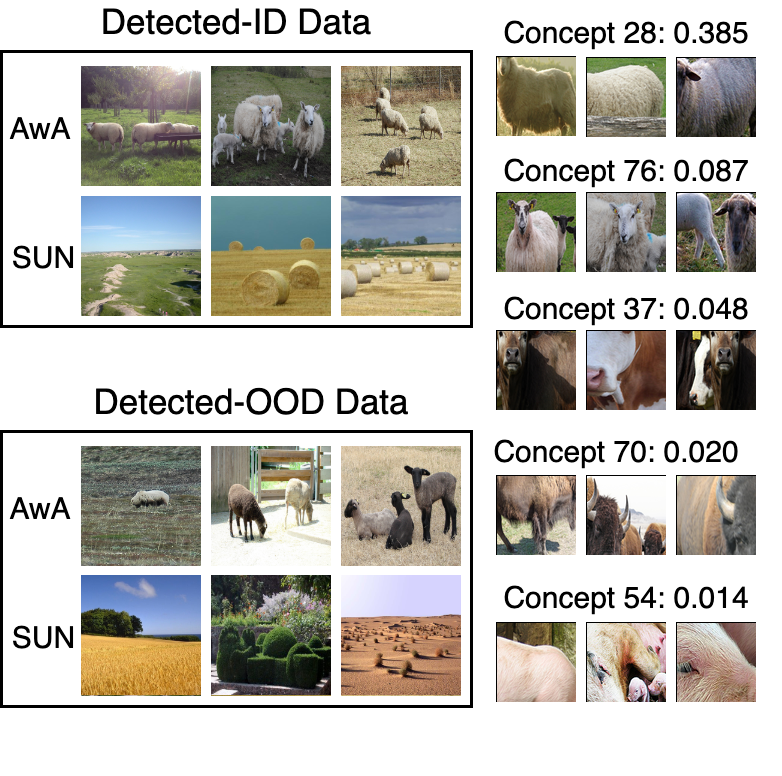
\includegraphics[scale=0.28]{figures/expl_sheep.png}
\vspace{-9mm}
\caption{\small \textbf{Top-6 important concepts for Energy with respect to class "Sheep".}
Concepts are obtained by our concept learning algorithm with $\lambda_\textrm{mse} = 1, \lambda_\textrm{norm} = 0.1, \lambda_\textrm{sep} = 0$.
To visualize what each concept represent, we display top receptive fields from $\Dinte$ whose inner product with the corresponding concept vector is above 0.8, along with the corresponding $\textrm{SHAP}(\eta^{j}_{\bff, S}, \bfc_i)$ value.}
\vspace{-5mm}
\label{fig:shap_sheep}
\end{figure}
\mypara{Contribution of each concept to detection.}
We address the following question: \textit{how much each concept contributes to OOD detection result?}
Recent works have suggested to adopt Shapley value from coalitional game theory literature \cite{shapley1953value,fujimoto2006axiomatic} to interpreting model predictions \cite{chen2018shapley,lundberg2017shapley,sundararajan2020shapley}.
Extending the idea, we modify Shapley value by incorporating our detection completeness metric (Eqn. (\ref{equ: completeness-detection})) as
\begin{align}
    \label{equ: ConceptSHAP}
    &\textrm{SHAP}(\eta^{}_{\bff, S}, 
    \bfc_i)  ~:= \nonumber \\
    &\sum_{\bfC' \subseteq \bfC \setminus \bfc_i} \frac{(m - |\bfC'| - 1)! |\bfC'|!}{m!} [\eta^{}_{\bff, S}(\bfC' \cup \{\bfc_i\}) - \eta^{}_{\bff, S}(\bfC')]
\end{align}
where $\bfC'$ is the subset of $\bfC$, and a high value represents the average marginal contribution of $\bfc_i$ across all possible coalitions when all classes are considered.
However, one might also want to assess the contribution of concepts to detection with respect to a particular class like "\textit{what concepts attribute to different detection results among the inputs predicted to the same class?}"
Thus, we can simply modify our detection completeness definition (Definition. (\ref{def:completeness_detec}) into its per-class variation by considering data that belong to a specific class $j$ as follows,
\begin{definition}
\label{def:completeness_detec_perclass}
Given a trained DNN classifier $\bff = \bfh \circ \bfphi$, a trained OOD detector with score function $S(\bfx, \bff)$, and a set of concept vectors $\bfC$, the {\em detection completeness score} with respect to ID distribution $\Pin(\bfx, y)$ and OOD distribution $\Pout(\bfx)$ is defined as
\begin{align}
\label{equ: completeness-detection-perclass}
    \eta^{j}_{\bff, S}(\bfC) 
    ~:=~ \frac{\textrm{sup}_\bfg \,\textrm{AUC}(\bfh \circ \recphi) ~-~ b_r}{\textrm{AUC}(\bfh \circ \bfphi) ~-~ b_r},
\end{align}
\end{definition}
% Note that for numerator we use predicted label -- don't have labels for OOD data. 
Accordingly, we use SHAP($\eta^{j}_{\bff, S}(\bfC)$) to denote SHAP($\eta^{}_{\bff, S}(\bfC) $) score specific to class $j$ where $\eta^{}_{\bff, S}(\bfC)$ is replaced in Eqn. (\ref{equ: completeness-detection-perclass}).
We show the top-ranked concepts by SHAP($\eta^{j}_{\bff, S}(\bfC)$) with respect to a specific class prediction in Figure \ref{fig:shap_sheep} (see Appendix \ref{sec:appendix-shapleys} for more results).
Also, we further investigate the attribution of such top-ranked concepts via counterfactual analysis (Appendix \ref{sec:appendix-counterfactual}).



% \mypara{Separability and interpretatbility}
% \begin{figure*}
%   \centering
%   \begin{tabular}{cc}
%     \subfloat[\label{fig:mnist}][Sampling distribution is skewed consistently for a single class (i.e. class 0)]
%     {
%     \hspace{-5mm}
%     \includegraphics[width=.49\linewidth]{mnist_class_0}} 
%     ~&~
%     \subfloat[\label{fig:asd}][Sampling distribution is skewed for the classes in turn (i.e. class 0, 1, 2, ...)]
%     {\includegraphics[width=.49\linewidth]{mnist_class_all}}
%   \end{tabular}
%   \caption{Accuracy vs training time-step in MNIST}
% \label{fig:mnist_results}
% \end{figure*}

\begin{figure*}[bt]
\centering
\subfloat[Set 1 with low concept separability, detected-ID \label{fig:low_in}]{\includegraphics[width=0.45\textwidth]{yeh_class17_AwA2_top10_detected_Energy.jpg}}\hfill
\subfloat[Set 2 with high concept separability, detected-ID \label{fig:high_in}] {\includegraphics[width=0.45\textwidth]{figures/ours_class17_AwA2_top10_detected_Energy.jpg}}\hfill\\
\vspace{-2mm}
\subfloat[Set 1 with low concept separability, detected-OOD \label{fig:low_out}]{\includegraphics[width=0.45\textwidth]{figures/yeh_class17_SUN_top10_detected_Energy.jpg}}\hfill
\subfloat[Set 2 with high concept separability, detected-OOD \label{fig:high_out}] {\includegraphics[width=0.45\textwidth]{figures/ours_class17_SUN_top10_detected_Energy.jpg}}
\caption{\small \textbf{Our concept separability metric and visual distinction in concept score patterns.} For class "Giraffe", we compare concept score patterns using different sets of concepts. \textbf{Left:} Averaged concept scores using concept set 1. \textbf{Right:} Averaged concept scores using concept set 2. For visualization of what each concept represents, see Appendix.}
\label{fig:high_separa_interpretatbility}
\end{figure*}
\mypara{Separability and interpretability}
Lastly, we use the concepts to gain insights on OOD detectors.
As shown in Figure \ref{fig:high_separa_interpretatbility}, we take the average of concept scores $V_{\textrm{in}}(\bfC')$ (or $V_{\textrm{out}}(\bfC')$) among the inputs that are predicted to class $j$, and detected as ID (or OOD) by OOD detector (\eg Energy in Figure \ref{fig:high_separa_interpretatbility}), where $\bfC'$ is the subset of original $m$ concepts $\bfC$. 
Here, we constitute the subset by taking the top-10 important concepts, ranked by their SHAP($\eta^{j}_{\bff, S}(\bfC)$) scores.
By comparing the patterns of averaged concept scores, one can understand how ID-detected inputs and OOD-detected inputs are different in terms of concepts, even when predicted to same class (compare Figure \ref{fig:low_in} vs. Figure \ref{fig:low_out}, or Figure \ref{fig:high_in} vs. Figure \ref{fig:high_out}).
Moreover, we confirm that a higher score for our concept separability metric enables more visual distinction  between concept score patterns.
For example, using concepts that yield relatively low per-class concept separability, $J^y_{\textrm{sep}}(\bfC')=0.059$, we fail to observe any noticeable difference in explanations between ID- and OO-detected data (see Figure \ref{fig:low_in} and \ref{fig:low_out}). 
On the other hand, concepts with high per-class concept separability, $J^y_{\textrm{sep}}(\bfC')=0.098$ successfully shows distinguishable pattern between ID- and OO-detected data (see Figure \ref{fig:high_in} and \ref{fig:high_out}). 
Such observation confirms our assumption that as long as classification completeness and detection completeness are preserved, having higher concept separability is beneficial for better interpretability for humans.
For further discussion, see Appendix \ryan{adding reminder to fill this in}.
